\documentclass{article}
\usepackage[utf8]{inputenc}
\usepackage{braket}
\usepackage{natbib}
\usepackage{graphicx}

\begin{document}

%%% Local Variables: ***
%%% mode:latex ***
%%% TeX-Master: "tesi-dott.tex"  ***
%%% End: ***
%%%%%%%%%%%%%%%%%%%%%%%%%%%%%%%%%%%%%%%%%%%%%%%%%%%%%%%%%%%%%%%%%%%
%
% Newcommand defintions
%
%%%%%%%%%%%%%%%%%%%%%%%%%%%%%%%%%%%%%%%%%%%%%%%%%%%%%%%%%%%%%%%%%%%
%
% Common colors
%
\newcommand{\cred}[1]{\textcolor{red}{#1}}
\newcommand{\cblue}[1]{\textcolor{blue}{#1}}
\newcommand{\cyellow}[1]{\textcolor{yellow}{#1}}
\newcommand{\ccyan}[1]{\textcolor{cyan}{#1}}
\newcommand{\cmage}[1]{\textcolor{magenta}{#1}}
\newcommand{\cgreen}[1]{\textcolor{green}{#1}}
\newcommand{\cblack}[1]{\textcolor{black}{#1}}
\newcommand{\cwhite}[1]{\textcolor{white}{#1}}
%
% Change the citation style
%
\makeatletter
\renewcommand{\@cite}[1]{
{$\!\! ^{(#1)}$}}
\makeatother
%{\renewcommand\@biblabel[1]{$^{#1}$}}
\renewcommand{\thefootnote}{\alph{footnote}}
\renewcommand{\thempfootnote}{\fnsymbol{mpfootnote}}
%\renewcommand{\showlabelsfont}{\small\slfamily}

%
%Slash aligned column 
%
\newcommand{\addtoc}[2]{\addcontentsline{toc}{#1}{\numberline{}#2}}
\newcommand{\etal}{{\emph{et al.}\ }}
\newcommand{\degr}{^{\circ}}

%
% Latin words
%
\newcommand{\Abinitio}{\emph{Ab initio}}
\newcommand{\abinitio}{\emph{ab initio}}
\newcommand{\invacuo}{\emph{in vacuo}}

%
% D2h and subgroups command
%
\newcommand{\Dtwoh}{\ensuremath{D_{2h}}}
\newcommand{\Ctwov}{\ensuremath{C_{2v}}}
\newcommand{\Ctwoh}{\ensuremath{C_{2h}}}
\newcommand{\Ctwo}{\ensuremath{C_{2}}}
\newcommand{\Ci}{\ensuremath{C_{i}}}
\newcommand{\Cs}{\ensuremath{C_{s}}}
\newcommand{\Dtwo}{\ensuremath{D_{2}}}
\newcommand{\Cone}{\ensuremath{C_{1}}}

%
% Some useful boxes
%
\newcommand{\cbw}[1]{\colorbox{white}{#1}}

\newcommand{\orbital}{\ensuremath{\varphi}}
\newcommand{\blockfunc}{\ensuremath{u}}
\newcommand{\density}{\ensuremath{\hat{\rho}}}
\newcommand{\nuclear}{\ensuremath{\hat{V}_{nuc}}}
%\newcommand{\coulomb}{\ensuremath{\hat{J}}}
\newcommand{\xc}{\ensuremath{\hat{V}_{xc}}}
\newcommand{\exchange}{\ensuremath{\hat{K}}}
\newcommand{\potential}{\ensuremath{\hat{V}}}
\newcommand{\kinetic}{\ensuremath{\hat{T}}}
\newcommand{\perturbation}{\ensuremath{\hat{h}}}
\newcommand{\effPot}{\ensuremath{v_{eff}}}
\newcommand{\nucPot}{\ensuremath{v_{nuc}}}
\newcommand{\elPot}{\ensuremath{v_{el}}}
\newcommand{\xcPot}{\ensuremath{v_{xc}}}
\newcommand{\fockMat}{\ensuremath{F}}
\newcommand{\fockOper}{\ensuremath{\hat{F}}}
\newcommand{\poisson}{\ensuremath{P(r-r')}}
\newcommand{\Poisson}[1]{\ensuremath{\hat{P}\Big[#1\Big]}}
\newcommand{\helmholtz}{\ensuremath{G^{\mu}(r-r')}}
\newcommand{\Helmholtz}[1]{\ensuremath{\hat{G}_i\left[#1\right]}}
\newcommand{\Helm}{\ensuremath{\hat{G}}}
\newcommand{\hamiltonian}{\ensuremath{\hat{h}}}
\newcommand{\pOper}{\ensuremath{\hat{p}}}

\newcommand{\pert}[2]{\ensuremath{#1^{(#2)}}}
\newcommand{\HopB}{\ensuremath{\pert{\hat{\boldsymbol{h}}}{B}}}
\newcommand{\HopM}{\ensuremath{\pert{\hat{\boldsymbol{h}}}{M_K}}}
\newcommand{\HopBB}{\ensuremath{\pert{\hat{\boldsymbol{h}}}{B,B}}}
\newcommand{\HopMB}{\ensuremath{\pert{\hat{\boldsymbol{h}}}{M_K,B}}}
\newcommand{\HopBM}{\ensuremath{\pert{\hat{\boldsymbol{h}}}{B,M_K}}}
\newcommand{\HmatB}{\ensuremath{\pert{\boldsymbol{h}}{B}}}
\newcommand{\HmatM}{\ensuremath{\pert{\boldsymbol{h}}{M_K}}}
\newcommand{\HmatBB}{\ensuremath{\pert{\boldsymbol{h}}{B,B}}}
\newcommand{\HmatMB}{\ensuremath{\pert{\boldsymbol{h}}{M_K,B}}}
\newcommand{\HmatBM}{\ensuremath{\pert{\boldsymbol{h}}{B,M_K}}}

\newcommand{\angmom}{\ensuremath{\boldsymbol{\hat{l}}}}
\newcommand{\rvec}{\ensuremath{\boldsymbol{r}}}

% Misc
\newcommand{\ud}{\ensuremath{\,\mathrm{d}}}

% Picture stuff
\newcommand{\defimgw}[2]{\pgfdeclareimage[width=#1]{#2}{#2}}
\newcommand{\defimgh}[2]{\pgfdeclareimage[height=#1]{#2}{#2}}

\newcommand*{\diff}{\mathop{}\!\mathrm{d}} % Differential
\newcommand*{\deriv}[3][]{% Derivative
\frac{\diff^{#1}#2}{\diff #3^{#1}}}

\newcommand{\scaling}{\ensuremath{\phi}}
\newcommand{\wavelet}{\ensuremath{\psi}}

\title{The MRChem MRA code for molecular electronic calculations. Performance and scaling properties}

\author{Peter Wind, Magnar Bjørve, Anders Brakestad, Luca Frediani, Gabriel Gerez, Stig Rune Jensen, Roberto Di Remigio}

%\affilition{Department of Chemistry, UiT - The Arctic University of Norway, N-9037 Tromsø, Norway}

\maketitle

\begin{abstract}
MRChem is a Multiresolution Analysis (MRA) code for molecular electronic calculations, based on a multiwavelets adaptive basis representation. A description of the implementation strategy is provided. Benchmark results on systems comprising more than thousand orbitals at the Hartree Fock (HF) level are analyzed, with an emphasis on scaling properties. 
We show that some terms which formally scale as $~0(N^2)$, in effect have a better scaling because of the implicit screening introduced by the inherent adaptivity of the method. Comparison with traditional GTO based software, show that MRChem can be competitive wrt computation time.

\end{abstract}

%test

\section{Introduction}


Gaussian basis sets (GTO and more generally Linear Combination of Atomic Orbitals, LCAO) are well established as a standard for ab initio molecular calculations. 
Even very small basis sets (a few functions per orbital) can give reasonable results for describing molecular properties. 

% Husker ikke om jeg skrev dette selv eller om det er tatt fra en artikkel!: In a localized orbital perspective, atom centered basis set are very effective to describe orbitals belonging to that atom, but are basis functions centered on other atoms will be much less useful for describing the local orbitals. For systems with many atoms, one ends up with describing orbitals with a large proportion of very small, coefficients. Those small parts are still necessary among other in order to ensure orthogonality among orbitals. The natural solution is then to describe different orbital or functions in different sets of basis functions. There are many problems associated with this approach, the main one is that each mathematical operation involving more than one function, must relate different basis sets and a new basis has to be defined for every new resulting function. It is a challenge to do this in a balanced and efficient way. 


In a MRA framework, the basis can adapt according to the function described (for an in-depth review of the MRA method in the field of Quantum Chemistry, see \citep[]{bischoff2019}). The available basis is in principle infinite, and the basis actually used is dynamically adapted to the required precision. However reasonable results can require the real-space basis to comprise millions of elements for each function. In this sense, the method starts with a big handicap, compared to Gaussian basis sets.

The challenge is not only the large amount of operations needed to perform calculations on large systems, but also the large memory footprint. Using a computer cluster, if not all the data can be stored locally, the data must be stored on separate compute nodes. On modern computers access to data is generally more time consuming than the mathematical operations itself, and if the data is not available locally, this is even more important. The implementation must be able to efficiently copy large amounts of data between compute nodes and the algorithm must be devised so as to use or reuse the data already locally available when possible.

With the exponential development of available computational resources, it has now become possible to perform such MRA calculations on systems comprising thousands of atoms \cite{ratcliff2020}, \cite{madness2016}. 

%For larger systems, or high precision, traditional basis set methods require large basis sets, as the same basis is used for all orbitals. Methods exists to "screen" the basis in order to use only a limited part of the entire basis, however the screening will only take effect if the corresponding part of the density matrix can be neglected. Higher accuracy requires larger basis sets, {\sl and} that a larger part of the space must be considered. For those systems the advantages of the Gaussian basis is not obvious.

In this article, we will present the main implementation features of a MRA code, MRChem, which at present is capable of describing systems with thousands of orbitals at the Hartree Fock or Density Functional Theory (DFT) level.  

The large memory requirement is addressed by storing the data in a distributed "memory bank", where orbitals can be sent and retrieved independently by any CPU. The total size of the memory bank is then only limited by total size available on the entire computer.

The large computational cost is addressed by parallelization either at the orbital level or through a partition of the real space. This  dual parallelization approach, allows to minimize the relative cost of communication and the overall computational costs.

The multiwavelet approach adapts the precision to the "smoothness" of the potential in a continuous way. The potential resulting from remote subsystems will locally be "smooth" and thereby only require a simplified (coarse grid) description. 

Using localized orbitals the adaptiveness of the multiwavelets description will reduce significantly the computational effort required to compute the terms that involves remote orbitals. This opens the way for a linearly scaling method where the linearity arises naturally from the methodology.


Benchmark calculations at the Hartree Fock level show that MRChem is able to describe systems with thousands of electrons, and exhibits near linear scaling properties. Computation times are competitive with state of the art traditional software.


\section{The multiwavelet method for Quantum Chemistry}

Only a superficial overview of the method is given here, as more detailed descriptions can be found elsewhere REF.

The Kohn Sham or HF equations can be written

\begin{equation}
  (-\frac{1}{2}\nabla^2 + V) \psi_i = \sum_{j_{occ}} F_{ij} \psi_j
\end{equation}

\begin{equation}
  F_{ij} = \langle \psi_i |{-\frac{1}{2}\nabla^2+V}| {\phi_j}\rangle
\end{equation}

In the HF case $V=V_n+J-K$, and in the Kohn Sham equations $V=V_n+J+V_{xc}$

Compared to more standard LCAO methods, there are a few limitations introduced by the wavelet approach:

Since the  MW functions are not continuous, derivation is problematic. The direct application of the kinetic operator, will not give an accurate result (but good approximations can be found [ref]).

In order to avoid direct use of the Kinetic operator one rewrite the equation as, 

\begin{equation}
\psi_i = -2 G_{i}(V\psi_i - \sum_{j_{occ} \ne i} F_{ij} \psi_j)
\end{equation}

where the Helmholtz operator $G_{i}$ is defined by
\begin{equation}
G_{i}(-\nabla^2 - 2 F_{ii} )=1
\end{equation}

Since the number of mw basis is not a priori limited, there is no natural way of defining a set of "virtual orbitals". We cannot define the Fock matrix in the entire basis and even less diagonalize it.


\subsection{Basic scf operations} %put complex conjugates!

We will here show the main steps involved in a SCF iteration in a mw framework.

First the matrix elements of the Fock operator are evaluated explicitly. This involves the application of the kinetic operator ($T$), nuclear  potential ($V_{nuc}$), Coulomb operator ($J$), and  the exchange potential ($K$) and/or the "exchange-correlation" potential from the density functional ($V_{xc}$) on each occupied orbital.

\subsubsection{$T$}
As mentioned the application of the kinetic operator on a mw function can be problematic. However first order derivatives are less problematic than second order derivatives. Further, since the matrix element involves an integration, the resulting numbers are in practice accurate enough. 
In our implementation the matrix elements are computed by first evaluating the first order derivative and the overlap between them:
\begin{equation}
  T_{ij} = -\frac{1}{2} \langle \nabla \psi_i |\nabla {\phi_j}\rangle
\end{equation}


\subsubsection{$V_{nuc}$}

The application of the nuclear potential (and possibly additional external fields) can be performed in two ways. Either the sum over nuclei is performed as a sum of matrix elements for the individual nuclei, or the sum over the potentials is performed first, and the matrix elements evaluated at the end. In our present implementation, the first form is used.
\begin{equation}
  V_{nuc} \phi_j = (\sum_{k = nuclei} V_k) \phi_j
\end{equation}
The total potential for all nuclei ($\sum_{k} V_k$) can be very large in terms of memory. It describes the potential over the entire space, whereas only the parts that overlap with the occupied orbitals are actually used. In the future we plan to adapt the accuracy according to the electronic density.

%The first expression is requires less operations, since only one operator application needs to be evaluated. The second form requires to apply an operator for each nucleus.

%However the second form may still have computational advantages:  The second form is also simpler to set into a parallel framework, since the contribution from each nucleus can be evaluated completely independently. The potential for a single nuclei is memorywise smaller than the total potential.

%I %but we should do something about it to reduce or delocalize the memory footprint

\subsubsection{$J$}

We compute the total density before the total Coulomb potential ($V_C$) is constructed and applied to the orbitals:

\begin{equation}
  V_{C}(r) = \int \frac{\sum_k \phi^*_k(r')\phi_k(r')}{|r-r'|} \ud r'
\end{equation}

\subsubsection{$K$}

The exchange terms are probably the most computationally demanding parts, because they require the application of the Coulomb operator for every orbital pair:

\begin{equation}
  K_{j} = \sum_k  K_{Ex}^k \phi_j 
\end{equation}
with 
\begin{equation}
  K_{Ex}^k(r) \phi_j = \phi_k(r) \int \frac{\phi^*_k(r')\phi_j(r')}{|r-r'|} \ud r'
\end{equation}

Section \ref{Xscreen} provides a more detailed description of how these terms can be evaluated efficiently. 

\subsubsection{$V_{xc}$}
In our implementation, the value of the density is evaluated at each point in space, and the dft potential is then evaluated using the external library XCfun[REF], and transformed back into a mw potential. 

\subsubsection{Helmholtz operator}

There is one Helmholtz operator associated to each orbital energy, however each Helmholtz operator is applied to a single orbital.

\subsubsection{Other}
In addition, the orbitals need to be orthonormalized, and combined (orbital rotation).

\subsubsection{Basic mw operations required}

The elementary mw operations required for all those steps are
\begin{itemize}
\item Construction of a mw function given an analytic or sampled function.
\item Evaluation of the value of a mw function at a given point in space.
\item Multiplication by a number.
\item Sum of two mw functions.
\item Product of two mw functions.
\item Overlap between two mw functions.
\item Application of a potential on a mw function (multiplication).
\item Evaluation (approximative) of the first order derivative of a mw function.
\item Application of Coulomb operator on a mw function to get a potential.
\item Construction and application of the Helmholtz operator.
\end{itemize}
All these operations are provided by the MRCPP library.

In addition the SCF requires schemes, for orthonormalization, localization and for making the guess of the next orbitals given the preceding iteration results (REF, KAIN).

\subsection{MRChem software, MRCPP and Vampyr}
%section about availability and things the code can do for the user
The MRChem code relies on the MRCPP library for performing the basic mathematical operations in a multiwavelet basis.

git, properties, Vampyr ...


\section{Implementation details and parallelization strategy}

MW calculations can be computationally demanding. Both the total amount of elementary operations and the large amount of memory required and the capacity of the network are important bottlenecks. 

In practice a computer cluster is required for calculations on large systems.
For example the representation of one orbital is described typically by of the order of 10-500MB of data (see section \ref{sizes}). Usually several sets of orbitals are required in the scf process (previous iteration, right hand size of equations etc.). If 1000 orbitals are described, this will often require more memory than is locally available on a compute node of a cluster. Therefore it is required to store the data in a distributed way. At the same time, the equations require to access all pair of orbitals, i.e. all the data must at some point be accessible locally.

In order to solve the equation in parallel, the problem needs to be partitioned into smaller parts that can be computed with as little transfer of data as possible between the different parts.



\subsection{Localized versus canonical orbitals}

Although localized and canonical orbitals represent the same wave function, the numerical operations required to solve the equations will have different scaling properties in a canonical or localized representation.
Because of the inherent adaptiveness of the mw approach, multiplying two orbitals, or applying an operator onto an orbital can be done more efficiently if the orbitala are localized in space. Even if the orbitals have non-negligible values in a large portion of space, the adaptiveness properties will make sure that the calculations in the parts where the orbitals are small are done at a coarser level of accuracy, and therefore faster than in the regions with larger values.


\subsection{Adaptivity and implicit screening}
%explanation of implicit screening mechanisms within MRA? 
% i.e. MRCPP tree calculation using norm threshold



\subsection{Local (real space) versus orbital representation}
%NB: easy to confuse real space local and localized orbitals!

The orbitals need to be stored on the computer. This can be done in several ways. The KS or HF equations are written in terms of orbitals, and therefore it is natural to implement the code in a way that follows the mathematical expressions, i.e. each orbitals is stored individually. Another way of partitioning the problem, is to consider one part of real space at a time, and store together the contributions from all the orbitals at that position. Both approaches have advantages and disadvantages.

However we will show here why it is advantageous, for some terms at least, to shift to a real-space partitioning approach.

(This is similar to the history for gaussian basis set methods, which started using Molecular Orbitals, but for large systems could get more efficient implementations by expressing the core terms using an "Atomic Orbitals" representation (Helgaker, T.; Jørgensen, P.; Olsen, J. Molecular Electronic-Structure Theory; John Wiley \& Sons, Ltd, 2014).)

In the computation of the Fock matrix elements, one has to evaluate terms of the form 

\begin{equation}
  {\hat O}_{ij} = \braket{\phi_i | {\hat O} |\phi_j}  = \braket{\phi_i | {\hat O} \phi_j} 
\end{equation}

where $\phi_i$ and $\phi_j$ are occupied orbital, and ${\hat O}$ is an operator, for example the nuclear potential operator. The application of the operator is a $~0(N)$ operation, and the calculations of the entire matrix scales formally as $~0(N^2)$. We can express explicitly the orbitals in the multiwavelet basis:

\begin{equation}
  \phi_i = \sum_{k,n} c_{ikn} p_{kn} 
\end{equation}
\begin{equation}
  {\hat O} \phi_j = \sum_{k,n} d_{jk_n} p_{kn} 
\end{equation}

where $p_{kn}$ is a member of the used mw basis, i.e. a three-dimensional polynomial (index $k$) for a multiwavelet node (index $n$) at specific position in space, and $c_{jkn}$ are the coefficients that define the function $\phi_j$ in that basis. 

Since the basis is adaptive, different functions will use different sets of nodes. 
In order to compute the overlap of two functions $\phi_i$ and $\phi_j$, they are first adaptively projected onto a common basis and multiplied.

\begin{equation}
  \braket{\phi_i|{\hat O} \phi_j} = \sum_{k_n} c_{ikn}d_{jkn}
\end{equation}

since $\braket{p_{kn}|p_{lm}} = \delta_{kl}\delta_{nm}$

This operation is equivalent to the multiplication of the $c$ and $d$ matrices. However for large systems, it is not possible to hold the coefficients for all the indices i,j,k,n in local memory.
The "MO" approach is then to sum over all $k,n$ for for each pair ij independently. The problem is that each coefficient $c_{jkn}$ is used only once at a time. On modern based computers memory access are much more time demanding (factor of the order of 100 for most CPU based systems) than the mathematical operations itself.  A much faster implementation is to consider a specific node n and perform the product for all i, j and k values within this node. 

\begin{equation}
  \braket{\phi_i | {\hat O} |\phi_j}_n = \sum_{k} d_{jkn} p_{kn} \forall i,j
\end{equation}

This results in a series of independent matrix multiplication operations that can fully utilize the capabilities of the computer. 

This means however that the storage of the orbitals in memory must be adapted. Instead of storing each orbital separately (orbital or MO representation), the values of all the orbitals at specific positions in space (node) must be easily accessible (local representation). To change from an orbital to a local representation is a $~0(N)$ operation,

It is still possible, to take advantage of the screening in the local approach: for each function, the norm values within each node is stored, so that when the product of the norms is below a threshold, the corresponding matrix multiplication does not need to be performed.

Also orbital rotations can be addressed in a similar way.

%which terms are using local storage

\subsection{MPI parallelization}

MRChem is parallelized using Message Passing Interface (MPI) and OpenMP.  

The MPI processes are partitioned into three groups:

\subsubsection{MPI "workers"} 
They perform the mathematical operations. These processes have also access to multiple threads for OpenMP parallelization. The large majority of the cores are assigned to worker processes.

The low level (operations on one or two orbitals or mw trees, and on nodes) are included  in the MRCPP library. The MRCPP will perform tree operations as a set of operations on nodes. Those operations will then be performed in parallel by OpenMP threads. The thread parallelity is transparent for the library user; only the number of threads needs to be set.


\subsubsection{Memory bank processes} 
These processes are only receiving and distributing data to the workers, they do not perform major mathematical operations and are not threaded. Those processes will impose a high load on the network; it is therefore important to distribute those process on all compute nodes in order to avoid saturation of the local network. Since the memory bank processes are different from the worker processes, the worker processes can access all the data without direct communication with other workers (in effect, one sided memory access). Efficient transfer of data is the key to a successful parallelization scheme.

In the multiwavelet approach, orbitals are functions represented in a tree structure. The root nodes cover the entire space of the system, and each subdivision defines branches. In order to facilitate the transfer of those functions, the tree structure and the node data are stored in piecewise contiguous memory. This allows the data to be sent efficiently among MPI processes: only the position in memory of the start and end are required, and some metadata information. A tree can then be transfered without intermediate buffering and with little overhead. 
The MRCPP library contains functionalities to easily and efficiently transfer mw trees (or orbitals) between MPI processes. 

The interface is simple and intuitive, and the basic commands in the C++ code are:
\begin{itemize}
    \item Save Orbital, give it an identification tag "id": 
    
put\_orb(id, Orbital)
\item Fetch Orbital with  identification tag "id": 

get\_orb(id, Orbital)

\end{itemize}


The underlying libraries will then find a suitable place in the "bank" to store the orbital.

%The MRCPP library allows to store a function as "shared memory" using MPI-3 functionalities. In such a format, all the MPI processes on a compute node can directly access a function using only one copy on the compute node. In our present implementation, the Nuclear and Coulomb potentials are stored in shared memory form.
%(We did not use the shared memory feature as much as intended, because we noticed that it sometimes causes a drop in performance, that was difficult to understand and control.)

\subsubsection{Task manager} 
In a localized orbital approach, many of the elements of the matrix $\braket{\phi_i|{\hat O} \phi_j}$ will be small. Since the method is inherently adaptive using the MRCPP library, the small elements will be faster to compute. In order to fully exploit this feature, a dynamical distribution of tasks is required.  
In practice the matrix $\braket{\phi_i|{\hat O} \phi_j}$ is partitioned into blocks. Each block represent one task to be performed by a "worker". When a "worker" is done with one task it can ask for a new task from the "task manager" until all the tasks are finished.

One single MPI process is reserved for managing the task queue. The only purpose of this process is to keep account of the tasks that have been assigned and the tasks left, and distribute unsolved tasks to the workers. It does only send and receive small amounts of data at a time (few bytes) and will therefore in practice not be saturated with requests.



%In a fixed and limited basis set, the functions and operators can be represented as dense arrays, and the mathematical expressions become matrix multiplications. Matrix multiplication can be performed very efficiently on all types of supercomputers (both CPU and GPU based).
%In the multiwavelet representation, the representation of functions are given in a different basis, and there is no simple way to represent the equations as dense matrix multiplications. Only at the node level, the polynomial representation is in a predefined basis, and this is exploited, but there are still too few polynomials to fully take advantage of the hardware. 

%in appendix? example of C++ command to fetch and store orbitals?

\subsection{Exchange screening}
\label{Xscreen}

The exchange terms require the evaluation of

\begin{equation}
\label{equ:ex}
  K_{Ex}^k(r) \phi_j = \phi_k(r) \int \frac{\phi^*_k(r')\phi_j(r')}{|r-r'|} \ud r'
\end{equation}

 for all $k$ and $j$

The evaluation of equation (\ref{equ:ex}) can be divided into 3 operations:
\begin{itemize}
\item Product of $\phi^*_k(r')$ and $\phi_j(r')$
\item Application of Poisson operator, $\int \frac{(\phi^*_k(r')\phi_j(r'))}{|r-r'|} \ud r'$
\item Product with $\phi_k(r)$, $\phi_k(r) (\int \frac{\phi^*_k(r')\phi_j(r')}{|r-r'|} \ud r')$
\end{itemize}

The application of the Poisson operator gives a long range potential that decreases as 1/r. However if the function $\phi_k(r)$ is localized, only the the part of the potential where $\phi_k(r)$ is large enough needs to be computed. More precisely the accuracy of the potential needs only to be computed up to a precision which is inverse proportional to the value of $\phi_k(r)$ at that point. 

To handle this situation, the Poisson operator can use an adaptive precision where the required precision of the operator application is determined locally by the value of a given function. In practice, a set of functions can be given, and the precision at a given node is determined by the largest value of the norm of those functions at this node. This allows to treat the two terms $\phi_k(r) \int \frac{\phi^*_k(r')\phi_j(r')}{|r-r'|} \ud r'$ and  $\phi_j(r) (\int \frac{\phi^*_k(r')\phi_j(r')}{|r-r'|} \ud r')$ using the same $\int \frac{\phi^*_k(r')\phi_j(r')}{|r-r'|} \ud r'$.  Also complex functions can take advantage of this symmetry, since the complex and real part of $\phi_k(r)$ can then use the same $\int \frac{\phi^*_k(r')\phi_j(r')}{|r-r'|} \ud r'$.

Without screening, the number of exchange terms grows as $N^2$ and each term requires the application of Poisson operator. Distant orbitals that do not overlap, do not contribute, and therefore proper handling of the screening will be reflected in a cost of the exchange terms that grows linearly in size for large enough systems (if the required overall absolute precision is held constant).



\subsection{$N_{occ}^3$ terms}

In our implementation there are two steps which require terms that scale with the third power of the number of (occupied) orbitals. 

The localization algorithm involves the product of dense matrices with sizes $N_{occ} \times N_{occ}$. 

The scheme for orthogonalization of orbitals uses the diagonalization of a hermitian matrix and subsequent matrix multiplications which both scales as $N_{occ}^3)$

Dense matrix operations can be performed extremely effectively on any computer, and those terms will not contribute significantly to the total computation time before considering sizes larger than roughly $N_{occ}=1000$ for serial matrix multiplications, or 10 to 100 thousand for parallel matrix multiplications (not yet implemented). 

Both steps are not specific to the multiwavelet approach, on the opposite, basis set approaches may require those steps to be performed on the virtual orbitals too. For large systems, it might also be possible to exploit the numerical sparsity of the matrices.

% In standard approaches the total number of basis functions has to be considered in the diagonalization steps ($0(N_{basis}^3)$). ?
% or ($0(N_{occ}^2 N_{basis})$ ? as claimed in
% The Journal of Chemical Physics 140, 204110 (2014); doi: 10.1063/1.4871876

\section{Benchmark results}

In this section we will show how MRChem performs for some simple systems of different size. MRChem is still under development and the results shown here are just a snapshot of the present situation. The goal is not to determine the limitations of the model, but rather to show that at least in some cases it behaves as intended and that the development is going the right way.

All the benchmark runs presented here were performed on "Betzy", a BullSequana XH2000 computer cluster, with 128 cores and 256 GiB memory per compute node, and infiniband HDR 100 interconnect REF?.

All times given in this section are subject to a significant imprecision. The reason for this are multiple. The runs have been executed in a MPI parallel framework on a supercomputer shared with other users. Several algorithms are performed with dynamic allocation of tasks; as a consequence the same calculations can have a different workload distributions in two repeated identical runs. The network capacity may also be affected by other users. In addition the time spent in different parts of the code may not be well defined: in a parallel framework the same code will start and end at different times for different processes. In principle the time for one block should include the time for all processes to be finished, however in practice processes are allowed to continue without waiting, until they need data which is not yet available.
The time for a similar SCF cycle may vary by less than 10\%. This accuracy should be sufficient for reflecting the main trends. 

\subsection{Scaling with system size}

\begin{figure}
\centering
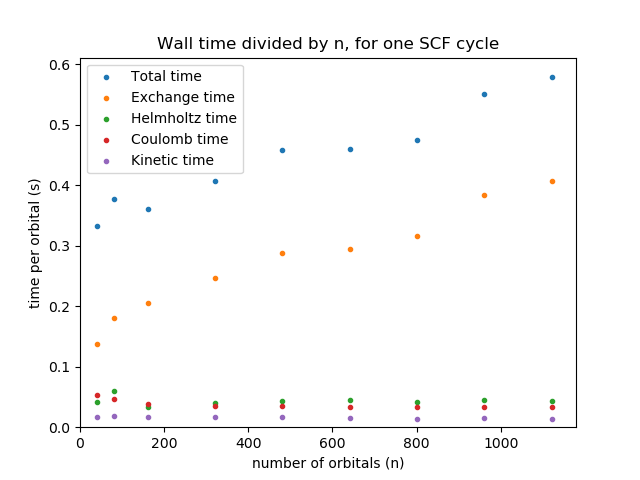
\includegraphics[width=1.\textwidth]{Times_nAlkanes.png}
\caption{\label{fig01}. Computation times divided by number of orbitals for one SCF cycle for different sizes alkanes: $C_{20}H_{42}$, $C_{40}H_{82}$, $C_{80}H_{162}$,$ C_{120}H_{242}$,$ C_{160}H_{322}$,$ C_{200}H_{402}$,$ C_{240}H_{482}$,$ C_{280}H_{562}$. Each molecule is computed using 8 compute nodes. Total time refers to the time spent in one Hartree-Fock SCF cycle, when it is close to convergence. Exchange time refers to the time spent for computing the Exchange contributions. Coulomb time refers to the time used for computing the Coulomb potential of each orbital, summing them up and distributing the total potential to all the compute nodes. Kinetic time refers to the time spent for computing the kinetic energy of each orbital  and Helmholtz time the time for constructing and applying the Helmholtz operator. Constant time per orbital would indicate linear scaling.}
\end{figure}

Figure \ref{fig01} show computation times divided by the number of orbitals for alkanes of different lengths. For a linear scaling method, the time per orbital should be approximately constant.  The time per orbital less than doubles going from the smallest (81 orbitals) to the largest (1121 orbitals) alkane. This shows that the scaling with system size is mostly linear, with a small non-linear contribution.  
% quadratic scaling would multiply the time by 13.8 

%The time consuming part of the Coulomb potential, is to gather the partial Coulomb potentials from each process, and distribute the total potential to all the processes again. The size (in terms of memory) of the potential will grow linearly with the size of the system. In addition the gather and scatter is done using a binary tree approach in our present implementation (this does not fully exploit the network parallelism, and better schemes can be implemented). The time for the Coulomb calculations is then formally growing as N ln2 N at present. In a local representation, this distribution of the full potential will not be necessary (but this is not yet implemented). At present the Coulomb and nuclear potential are treated independently. Since they largely cancel each other, a better approach would be to consider the sum of them directly, at least for remote nuclei and orbitals.

%The smallest alkanes are not able to make an optimal utilization of all the available cpus

The clearly most time consuming term is the exchange term. The other terms are showing close to linear scaling properties.

The number of non-negligible exchange contributions should ideally grow linearly with system size for large enough systems, and therefore the exchange computation time per orbital should be constant. However exchange contributions are the result of a sum of terms, and if the number of terms increase the accuracy of each individual term must be increased in order to achieve a fixed absolute precision in the final result. In our implementation, this is taking care of by increasing the required precision of the individual terms by a factor proportional to the square root of the number of orbitals. This is the main reason why our run times are not exhibiting a clearer linear trend.


\subsection{Size of orbital representation}
\label{sizes}

In a localized approach, the shape of the orbitals generally do not depend on remote atoms. In a direct basis set approach (if no special filtering is applied) the representation of an orbital will span the entire represented space, since the basis will increase with the system size. In the multiwavelet approach the orbital will essentially be represented using locally defined functions.
This is confirmed in our calculations.
The individual size of the orbitals, will of course vary greatly according to the type (core orbitals are simpler and therefore require less data to represent at a given precision, more diffuse function have more features than require more data to describe). As an illustration, in the molecules presented here, the largest orbital may be two to four times larger than the average, and the smallest a third of the average size.

The number of orbitals together with the size of the orbitals can be seen as an indicator of how much computational resources (memory, cpu time, and network) are required to solve the equations. 

\begin{table*}[t]
    \centering
    \begin{tabular}{cccccccccc}
& $C_{20}H_{42}$& $C_{40}H_{82}$& $C_{80}H_{122}$& $C_{120}H_{242}$&  $C_{200}H_{442}$ & $C_{280}H_{562}$ &valinomycine & gramicidin\\
orbital size (MB)  &  39 &  40   & 43  &  45  & 46 & 47 & 50 & 53\\
    \end{tabular}
    \caption{Average orbital size of different molecules (1e-5 prec). The average orbital size (in terms of number of nodes or coefficients) of the alkanes series is almost independent of the size of the molecule for the largest sizes}
    \label{tab:orbsizes}
\end{table*}



\subsection{Scaling with precision}

In table \ref{tab:prec} we have performed calculations with different precisions on two molecules, valinomycine (300 orbitals) and the gramicidin dimer (1008 orbitals).


\begin{table*}[t]
\label{tab:prec}
    \centering
    \begin{tabular}{cccccccccc}
&orbital size& Exchange &  Coulomb & Kinetic energy& Helmholtz & Total \\
 Valinomycine 1E-5& 49 & 71.4& 9.2& 2.7 & 7.4& 97.4\\
Valinomycine 1E-6& 115 & 182.4& 25.3& 6.7 & 21.3&251.2\\
Valinomycine 1E-7& 245 & 442.8& 78.8&17.1& 66.4&644.4  \\
%Valinomycine &1E-8  & 531.0& 163.9& 12.9&32.7& 852.6 \\ older run, different setup
 Gramicidin 1E-5&55&115&18& 4& 8& 164\\
  Gramicidin 1E-6&136&312 & 46& 15 & 26& 429\\
  Gramicidin 1E-7&306& 813&126& 28& 82& 1131\\ %cycle 4
    \end{tabular}
    \caption{Time (in seconds) for different terms in the SCF cycle. Valinomycine using 16 compute nodes and gramicidin 64 compute nodes. The average size (in MB) for one orbital is also given.} %times for cycle 6. 12 MPI/cnode, 4 bank/cnode, 15 OMP
    \label{tab:times}
\end{table*}

We observe roughly a factor of 2.5 increase in computation times for each increase by a factor of ten of the precision. 
An increase in the number of coefficients describing the orbitals will clearly increase the computational cost of each operation using this orbital. In addition an increase in precision will also extend the range of orbitals with non-negligible interactions, i.e. gives less effective screening.



\subsection{Implicit screening}
%example of histogram of timing for each exchange terms? many terms very fast, few slow.
%example of histogram of timing for orbital rotation?

\subsection{Comparison with ORCA REF and LSDalton REF}
\begin{table*}[t]
    \centering
    \begin{tabular}{lllll}
     & E [a.u.] &$\Delta$E [a.u.]& Error [a.u.] & time [s]\\
    LSDalton pc-1 &-3770.20554&-19.12076&0.11&101\\
    LSDalton pc-2 &-3772.56656&-19.27598&-0.04&1688\\
    LSDalton pc-3 &-3772.833116&-19.24894&-0.014&26319\\
    LSDalton$^+$ pc-3 &-3772.82592&-19.26353&-0.029&1924\\
    ORCA pc-1 &-3770.19956&-19.11479&0.12&25\\
    ORCA pc-2 &-3772.56922&-19.27865&-0.044&265\\
    ORCA pc-3 &-3772.83357&-19.24940&-0.014&3933\\
    MRChem mw4&-3772.85028&-19.21937&0.015&117\\
    MRChem mw5&--3772.86560&-19.23469&0.00025& 97$^*$\\
    MRChem mw6&3772.86584&-19.234934&0.00001&251$^*$\\
    MRChem mw7&-3772.86585&-19.234944&0&644$^*$\\
       \end{tabular}    
    \caption{Comparison of results and computation times, for one SCF cycle (Hartree Fock, Valinomycine molecule). LSDalton$^+$ is performed using the accelerators "DENSFIT" and "ADMM". E is the total Hartree fock Energy and $\Delta$E is the atomization energy. The error is defined as the difference with the mw7 results. time is the wall time for one scf cycle. $^*$All computation where done on 4 compute nodes, except for MRChem mw5, mw6 and mw7 which were performed using 16 compute nodes}
        \label{tab:MRC_ORCA_LSD}
\end{table*}

Table \ref{tab:MRC_ORCA_LSD} shows the computation time for one SCF cycle for the Valinomycine molecule computed at the Hartree Fock level. The accuracy of the total energy and atomization energies are compared with the ORCA and LSDalton
results using a pc-1, pc-2 and pc-3 basis set (the pc-4 basis was out of reach). 

Even at the lowest precision (mw4), the results have the same quality as the pc-3 basis, but at a fraction of the computational cost. 

It should be noted that the run times given for ORCA and LSDalton could probably be improved by tuning different input parameters, as we did not try to further optimize all the settings. Still the main picture should not be affected.




% comparison with linearly scaling methods?

\section{Discussion}
We have presented a fully functional implementation of the multiwavelet method and demonstrated that it is capable of handling systems with thousands of electrons at the Hartree Fock (or DFT) level. The scaling with system size is almost linear. There are certainly many alternative ways to approach the problem and we still expect that significant improvements in the efficiency of the algorithm will be implemented in the coming years. 

Specially the large memory footprint is a serious bottleneck that should be improved. %could be quantified: how large fraction of the coefficients are actually not negligible

It is remarkable that even if the actual basis used in MRChem can be several order of magnitudes larger than what is used in large GTO basis, the computation times are still competitive. We believe this is due to the fact that modern computers are extremely efficient when it comes to performing a large number of mathematical operations simultaneously, and the parts which are most time consuming are usually the transfer of data from main memory into cache, and transfer of data between compute nodes. The ability to partition the problem into independent parts is becoming more important than minimizing the overall number of mathematical operations. In this respect, the MRA framework has an advantage because of the orthogonality of the initial basis. See also the discussion about the relationship between HPC and Computational Chemistry in \cite{penchoff2021} and \cite{ratcliff2016}.

Also for DFT methods, it has already been shown (Bischoff 2019) that MRA methods can be competitive wrt computation time.

%Optimizing large computations has two complementary sides: on one hand the code should use efficiently the hardware available (CPU, network, memory) and on the other hand, the code should be able to scale to a large number of CPUs. In our approach we have mainly focused on the second part so far, since modern supercomputer are growing exponentially in size (Moore's law), and we expect in the future the main limitation to be the ability of software to make use of this large sizes, rather than to use them optimally.


For low or medium precision, the computer resources required are still larger than traditional basis set approaches. The results obtained with our implementation show that for higher precision the wavelet approach is competitive in term of computation times.

%to be expanded?
The ability to better control precision is a definitive advantage of the method. 



It is fair to say that finite basis set method benefit from decades of development by thousands of scientists, while only a few groups are actually developing multiwavelet methods for quantum chemistry calculations. We can therefore expect that the potential for further optimizations of the method and extension of the range of application will still increase widely in the future. %correlated methods?


\section{acknowledgements}
SIGMA2, nn9330k, Hylleraas



\bibliographystyle{plain}
\bibliography{references}

Goedecker, S. (1999). Linear scaling electronic structure methods. Reviews of Modern Physics, 71(4), 1085–1123. doi:10.1103/revmodphys.71.1085 

BigDFT method
https://aip-scitation-org.mime.uit.no/doi/full/10.1063/1.2949547

Real space methods:
 DOI: 10.1039/C5CP90198G (Editorial) Phys. Chem. Chem. Phys., 2015, 17, 31357-31359
Real-space numerical grid methods in quantum chemistry
Luca Frediani and Dage Sundholm
https://pubs.rsc.org/en/content/articlehtml/2015/cp/c5cp90198g?page=search


MP2:
https://aip.scitation.org/doi/10.1063/1.5141880
Direct determination of optimal pair-natural orbitals in a real-space representation: The second-order Moller–Plesset energy
 J. Chem. Phys. 152, 074105 (2020); https://doi.org/10.1063/1.5141880
Jakob S. Kottmann1,a), Florian A. Bischoff1,b), and Edward F. Valeev

%Predictive computation of properties of molecules and materials requires a highly precise numerical representation of many-body electronic wave functions/operators. Accurate electronic wave functions, such as in the coupled-cluster method, are traditionally represented in the Linear Combination of Atomic Orbitals (LCAO) representation using pre-optimized sequences of atom-centered basis sets (represented by analytic Gaussian-type or Slater-type functions, or represented numerically1). Recently, many-body electronic structure computations have also been demonstrated in the (augmented) plane-wave (PW) representation.2 Both representations suffer from slow convergence to the basis set limit, requiring the use of basis set extrapolation3,4 or explicit correlation.5,6 Although it is possible to closely match experimental chemical energy differences, such as atomization energies of small molecules,7 with the LCAO approaches, such computations suffer from high cost and poor conditioning and do not lend themselves to fast (reduced-scaling) reformulation due to the fully dense representation of electronic states and operators. The known bias of common AO basis sets toward ground-state energies makes it difficult to attain similar accuracy for excited states and response properties. Meanwhile, the plane wave representation struggles with the description of position-localized (e.g., intra-atomic) features of the electronic wave functions and thus also do not naturally lend themselves to low-order formulations.
%Grid-based real-space numerical representations of many-body wave functions, such as finite difference and finite/spectral elements, provide an alternative to the LCAO and PW representations with a number of attractive features, such as the ability to resolve spatially localized features, systematic bias-free improvability, and good conditioning. The main bottleneck to routine use of such representations is the impractical size of the 3k-dimensional grid needed to represent a k-particle state. Even pair theories (k = 2) such as MP2 and CCSD become prohibitively expensive for molecular systems due to the grid size; only symmetry-based dimension reduction in atoms makes the application of pair theories possible.8–12

\begin{thebibliography}{}


\bibitem[Bischoff (2019)]{bischoff2019}Florian A. Bischoff https://doi.org/10.1016/bs.aiq.2019.04.003  Computing accurate molecular properties in real space using multiresolution analysis,  2019

\bibitem[Ratcliff (2020)]{ratcliff2020}Laura E. Ratcliff,  William Dawson2, Giuseppe Fisicaro, Damien Caliste, Stephan Mohr, Augustin Degomme, Brice Videau, Viviana Cristiglio, Martina Stella, Marco D’Alessandro, Stefan Goedecker, Takahito Nakajima2, Thierry Deutsch, and Luigi Genovese J. Chem. Phys. 152, 194110 (2020) https://doi.org/10.1063/5.0004792 Flexibilities of wavelets as a computational basis set for large-scale electronic structure calculations

\bibitem[Harrison (2016)]{madness2016}R. J. Harrison, G. Beylkin, F. A. Bischoff, J. A. Calvin, G. I. Fann, J. Fosso-Tande, D. Galindo, J. R. Hammond, R. Hartman-Baker, J. C. Hill, J. Jia, J. S. Kottmann, M.-J. Yvonne Ou, J. Pei, L. E. Ratcliff, M. G. Reuter, A. C. Richie-Halford, N. A. Romero, H. Sekino, W. A. Shelton, B. E. Sundahl, W. S. Thornton, E. F. Valeev, Á. Vázquez-Mayagoitia, N. Vence, T. Yanai, and Y. Yokoi, SIAM J. Sci. Comput. 38, S123 (2016). https://doi.org/10.1137/15m1026171

\bibitem[Ratcliff (2016)]{ratcliff2016}Laura E. Ratcliff, Stephan Mohr, Georg Huhs, Thierry Deutsch, Michel Masella, Luigi Genovese  https://doi.org/10.1002/wcms.1290 Challenges in large scale quantum mechanical calculations


\bibitem[penchoff (2021)]{penchoff2021}https://pubs.acs.org/doi/full/10.1021/bk-2021-1388.ch001  HPC challenges: An Introduction to High Performance Computing and Its Intersection with Advances in Modeling Rare Earth Elements and Actinides

\end{thebibliography}
\end{document}
